\section{Introduction}
\begin{frame}{}
    \LARGE SSL: \textbf{Introduction}
\end{frame}

\begin{frame}[allowframebreaks]{Introduction}
    \begin{figure}
        \centering
        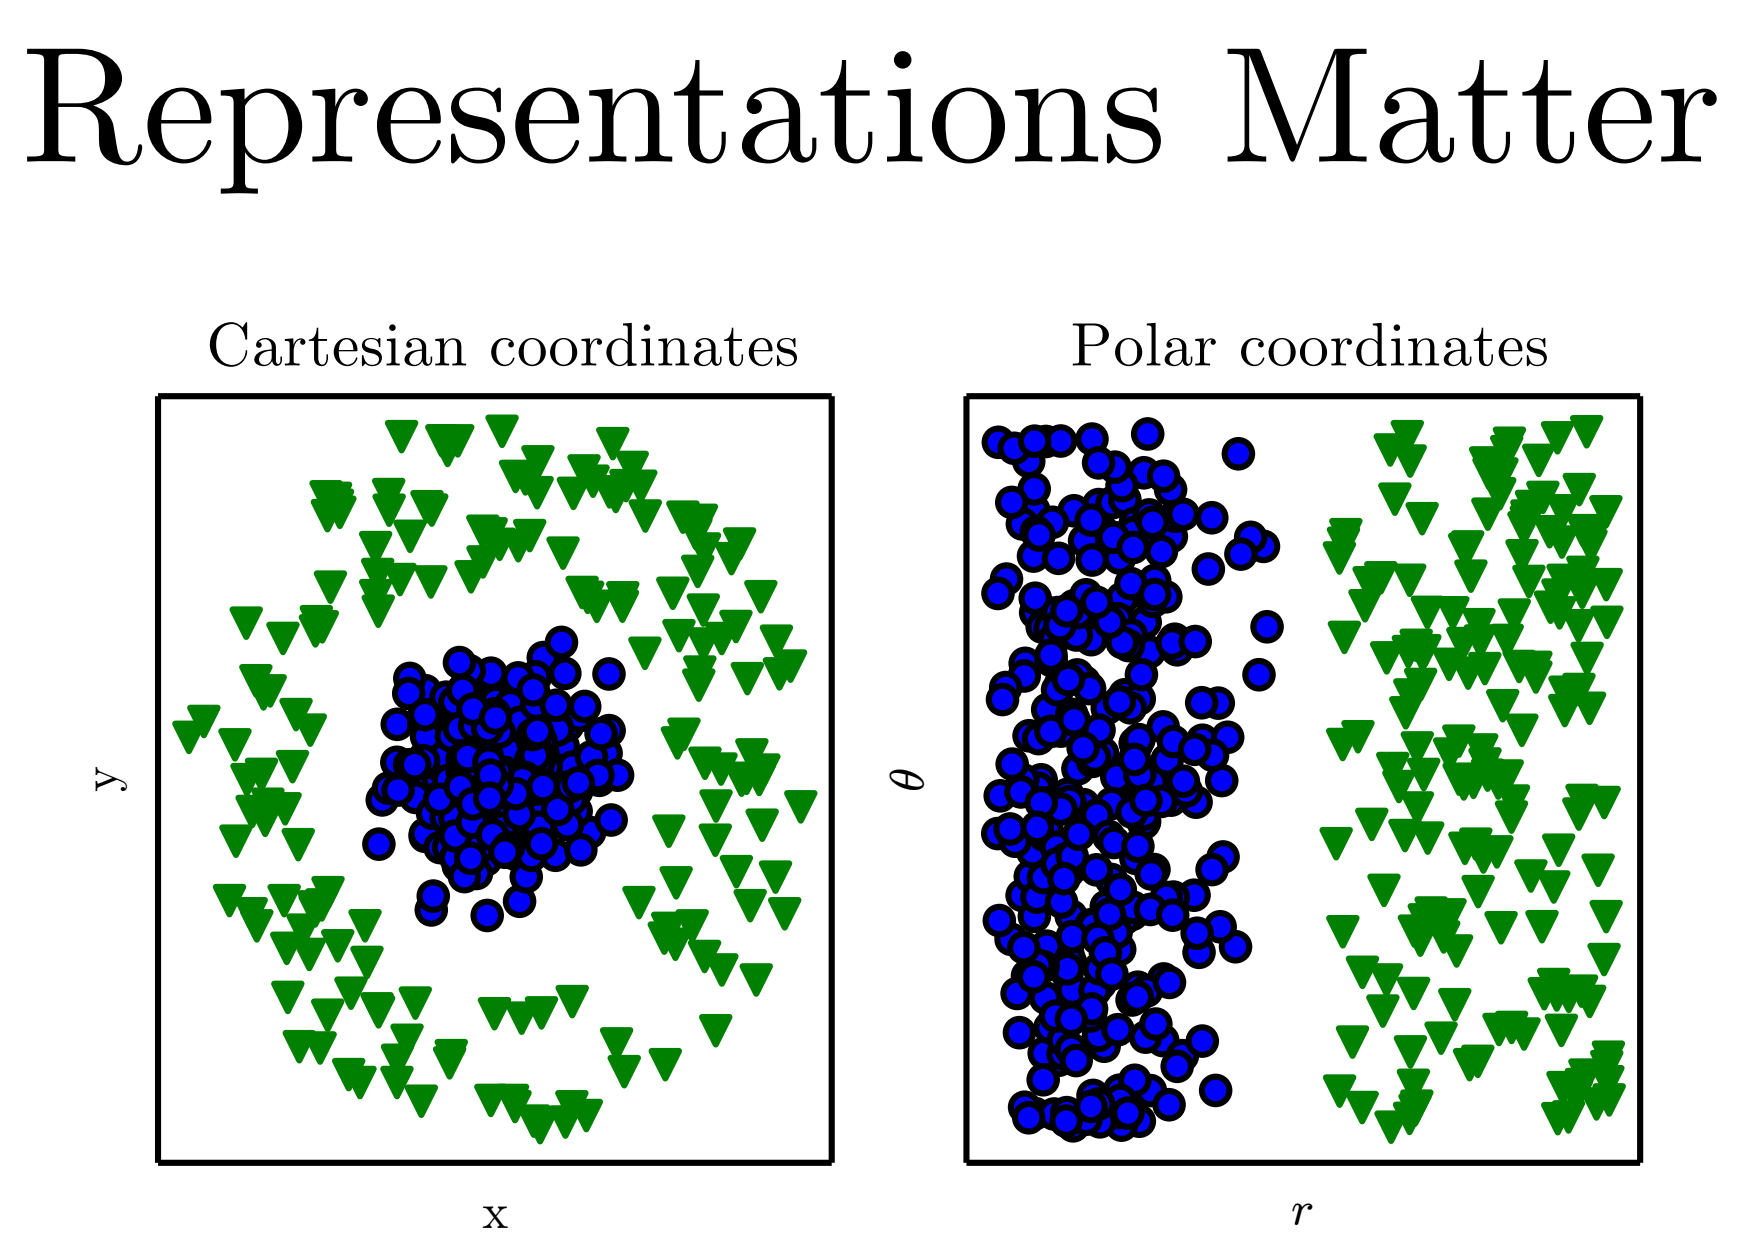
\includegraphics[width=\linewidth,height=0.9\textheight,keepaspectratio]{images/ssl/slide_2_1_img.png}
    \end{figure}

    \framebreak

    \begin{columns}
    \begin{column}{0.7\textwidth}
        \begin{figure}
            \flushleft
            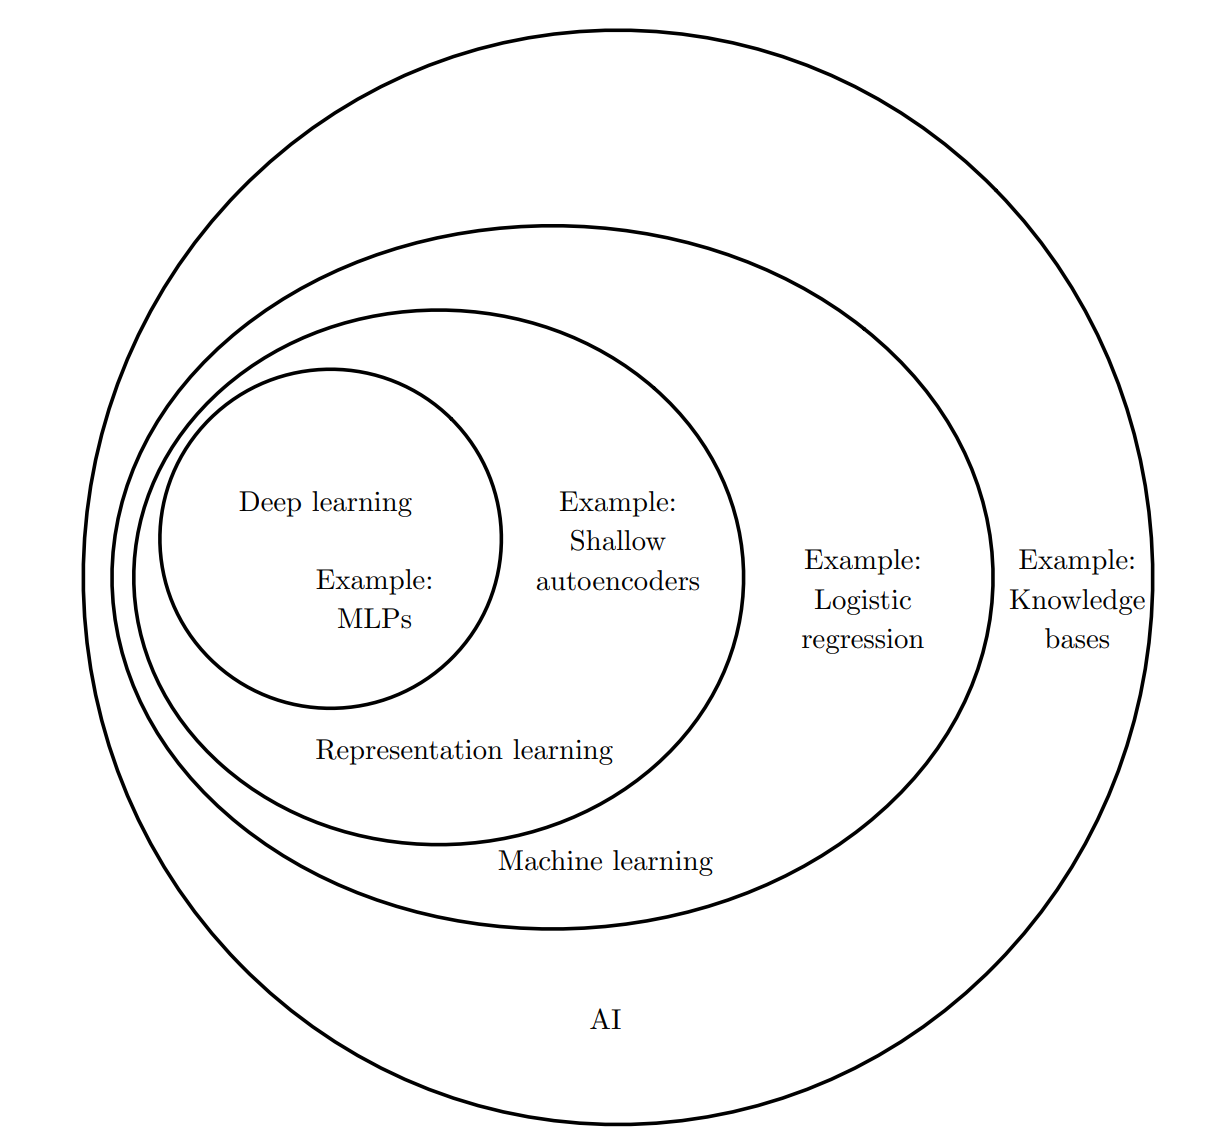
\includegraphics[width=\linewidth,height=0.8\textheight,keepaspectratio]{images/ssl/slide_3_1_img.png}
        \end{figure}
    \end{column}
    \begin{column}{0.48\textwidth}
        \textbf{Deep Unsupervised Learning:}
        \begin{itemize}
            \item Learns data representations without using labels.
            \item Is a subset of Deep Learning, which itself is a subset of Representation Learning, all within Machine Learning.
        \end{itemize}
    \end{column}
    \end{columns} 
    
    \framebreak

    \begin{columns}
    \begin{column}{0.55\textwidth}
        \begin{figure}
            \flushleft
            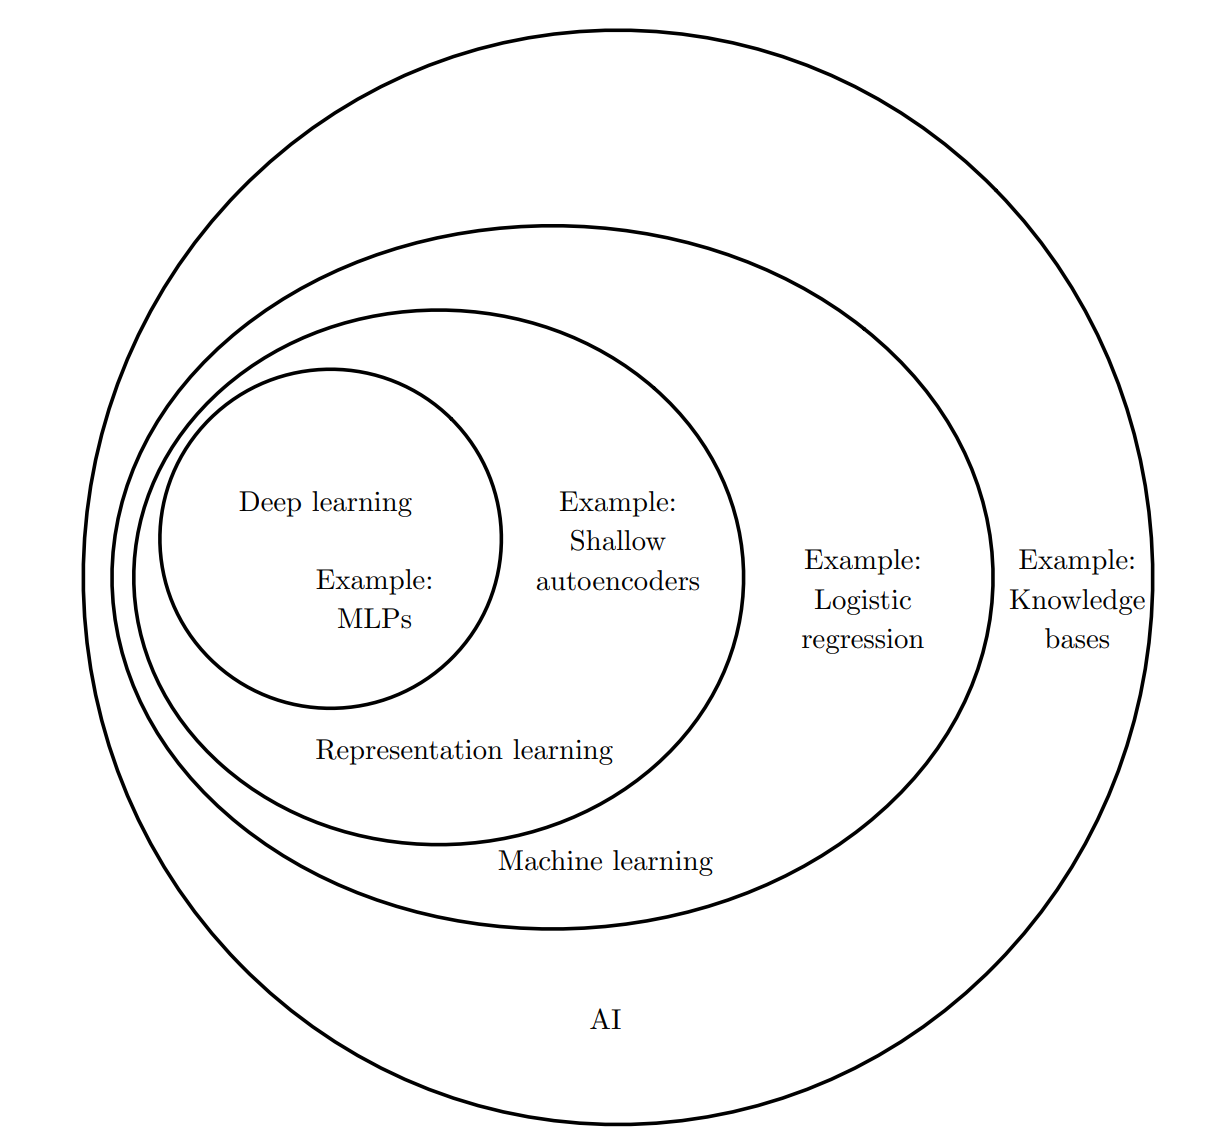
\includegraphics[width=\linewidth,height=0.8\textheight,keepaspectratio]{images/ssl/slide_3_1_img.png}
        \end{figure}
    \end{column}
    \begin{column}{0.62\textwidth}
        \textbf{Deep Unsupervised Learning:}
        \begin{itemize}
            \item Learns data representations without using labels.
            \item Is a subset of Deep Learning, which itself is a subset of Representation Learning, all within Machine Learning.
        \end{itemize}
        \vspace{0.5em}
        \textbf{Self-Supervised Learning (SSL):}
        \begin{itemize}
            \item A form of unsupervised learning that creates supervision from the data itself by designing \textit{pretext tasks}.
            \item These tasks generate pseudo-labels, enabling the model to learn useful representations without manual annotation.
            \item Often used interchangeably with unsupervised learning, but SSL specifically focuses on leveraging intrinsic data structure.
        \end{itemize}
    \end{column}
    \end{columns} 
\end{frame}

\begin{frame}[allowframebreaks]{Why Self-Supervised Learning?}
    \begin{itemize}
        \item \textbf{High cost of dataset creation:} Each new task often requires building a new labeled dataset.
        \begin{itemize}
            \item Involves preparing labeling manuals, defining categories, hiring annotators, building GUIs, and managing storage pipelines.
        \end{itemize}
        \item \textbf{Expensive supervision:} High-quality labels can be costly or impractical to obtain (e.g., in medicine or legal domains).
        \item \textbf{Leverage unlabeled data:} The internet provides vast amounts of unlabeled images, videos, and text that can be utilized.
        \item \textbf{Cognitive motivation:} Animals and babies learn from their environment without explicit supervision, inspiring SSL approaches.
    \end{itemize}

    \framebreak

    \begin{columns}
    \begin{column}{0.7\textwidth}
        \begin{figure}
            \flushleft
            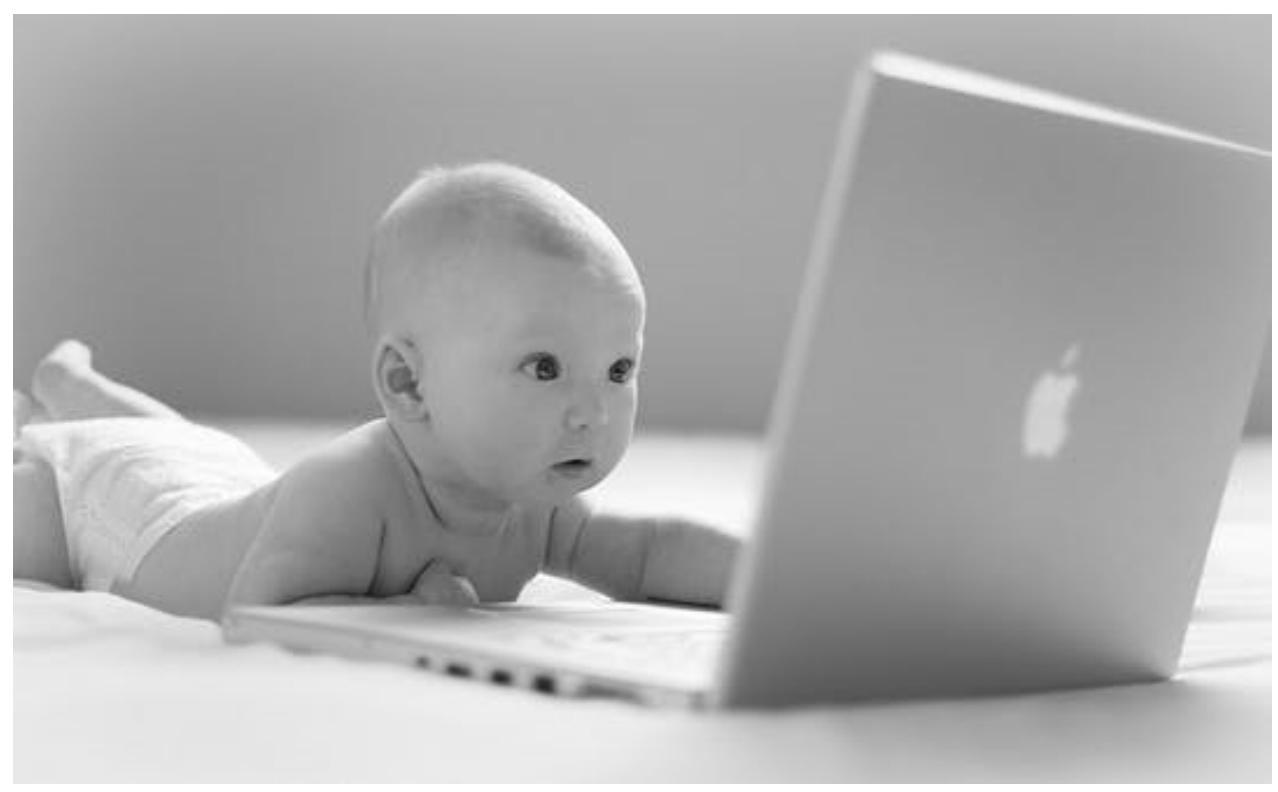
\includegraphics[width=\linewidth,height=0.8\textheight,keepaspectratio]{images/ssl/slide_7_1_img.png}
        \end{figure}
    \end{column}
    \begin{column}{0.4\textwidth}
        \textit{“Give a robot a label and you feed it for a moment; teach a robot to label and you feed it for a lifetime.”} \\
        \hspace*{\fill}--- Pierre Sermanet

        \vspace{1em}

        \small
        This quote highlights the core motivation behind self-supervised learning
        
        $\rightarrow$ enabling machines to generate their own supervision from data

        $\rightarrow$ thus reducing reliance on costly manual labeling and
        
        $\rightarrow$ fostering scalable, autonomous learning.
    \end{column}
    \end{columns} 
\end{frame}

\begin{frame}[allowframebreaks]{What is Self-Supervised Learning?}
    SSL is a type of unsupervised learning where the data itself provides supervision. Typically, part of the data is hidden, and a neural network is trained to predict it from the rest—this defines the \textit{pretext task}. Well-chosen pretext tasks help models learn useful features without manual labels.

    \begin{itemize}
        \item \textbf{Pretext Task}: Examples include predicting masked patches, future representations (CPC), or distinguishing positive/negative pairs (contrastive).
        \item \textbf{Downstream Task}: After pre-training, the encoder is fine-tuned for tasks like classification or detection.
        \item \textbf{Key Trade-Offs}:
        \begin{itemize}
            \item \textbf{Reconstructive} (e.g., autoencoders): capture low-level details, may miss semantics.
            \item \textbf{Predictive/Contrastive} (e.g., CPC, MoCo): focus on high-level information.
        \end{itemize}
    \end{itemize}

    \framebreak

    \begin{figure}
        \centering
        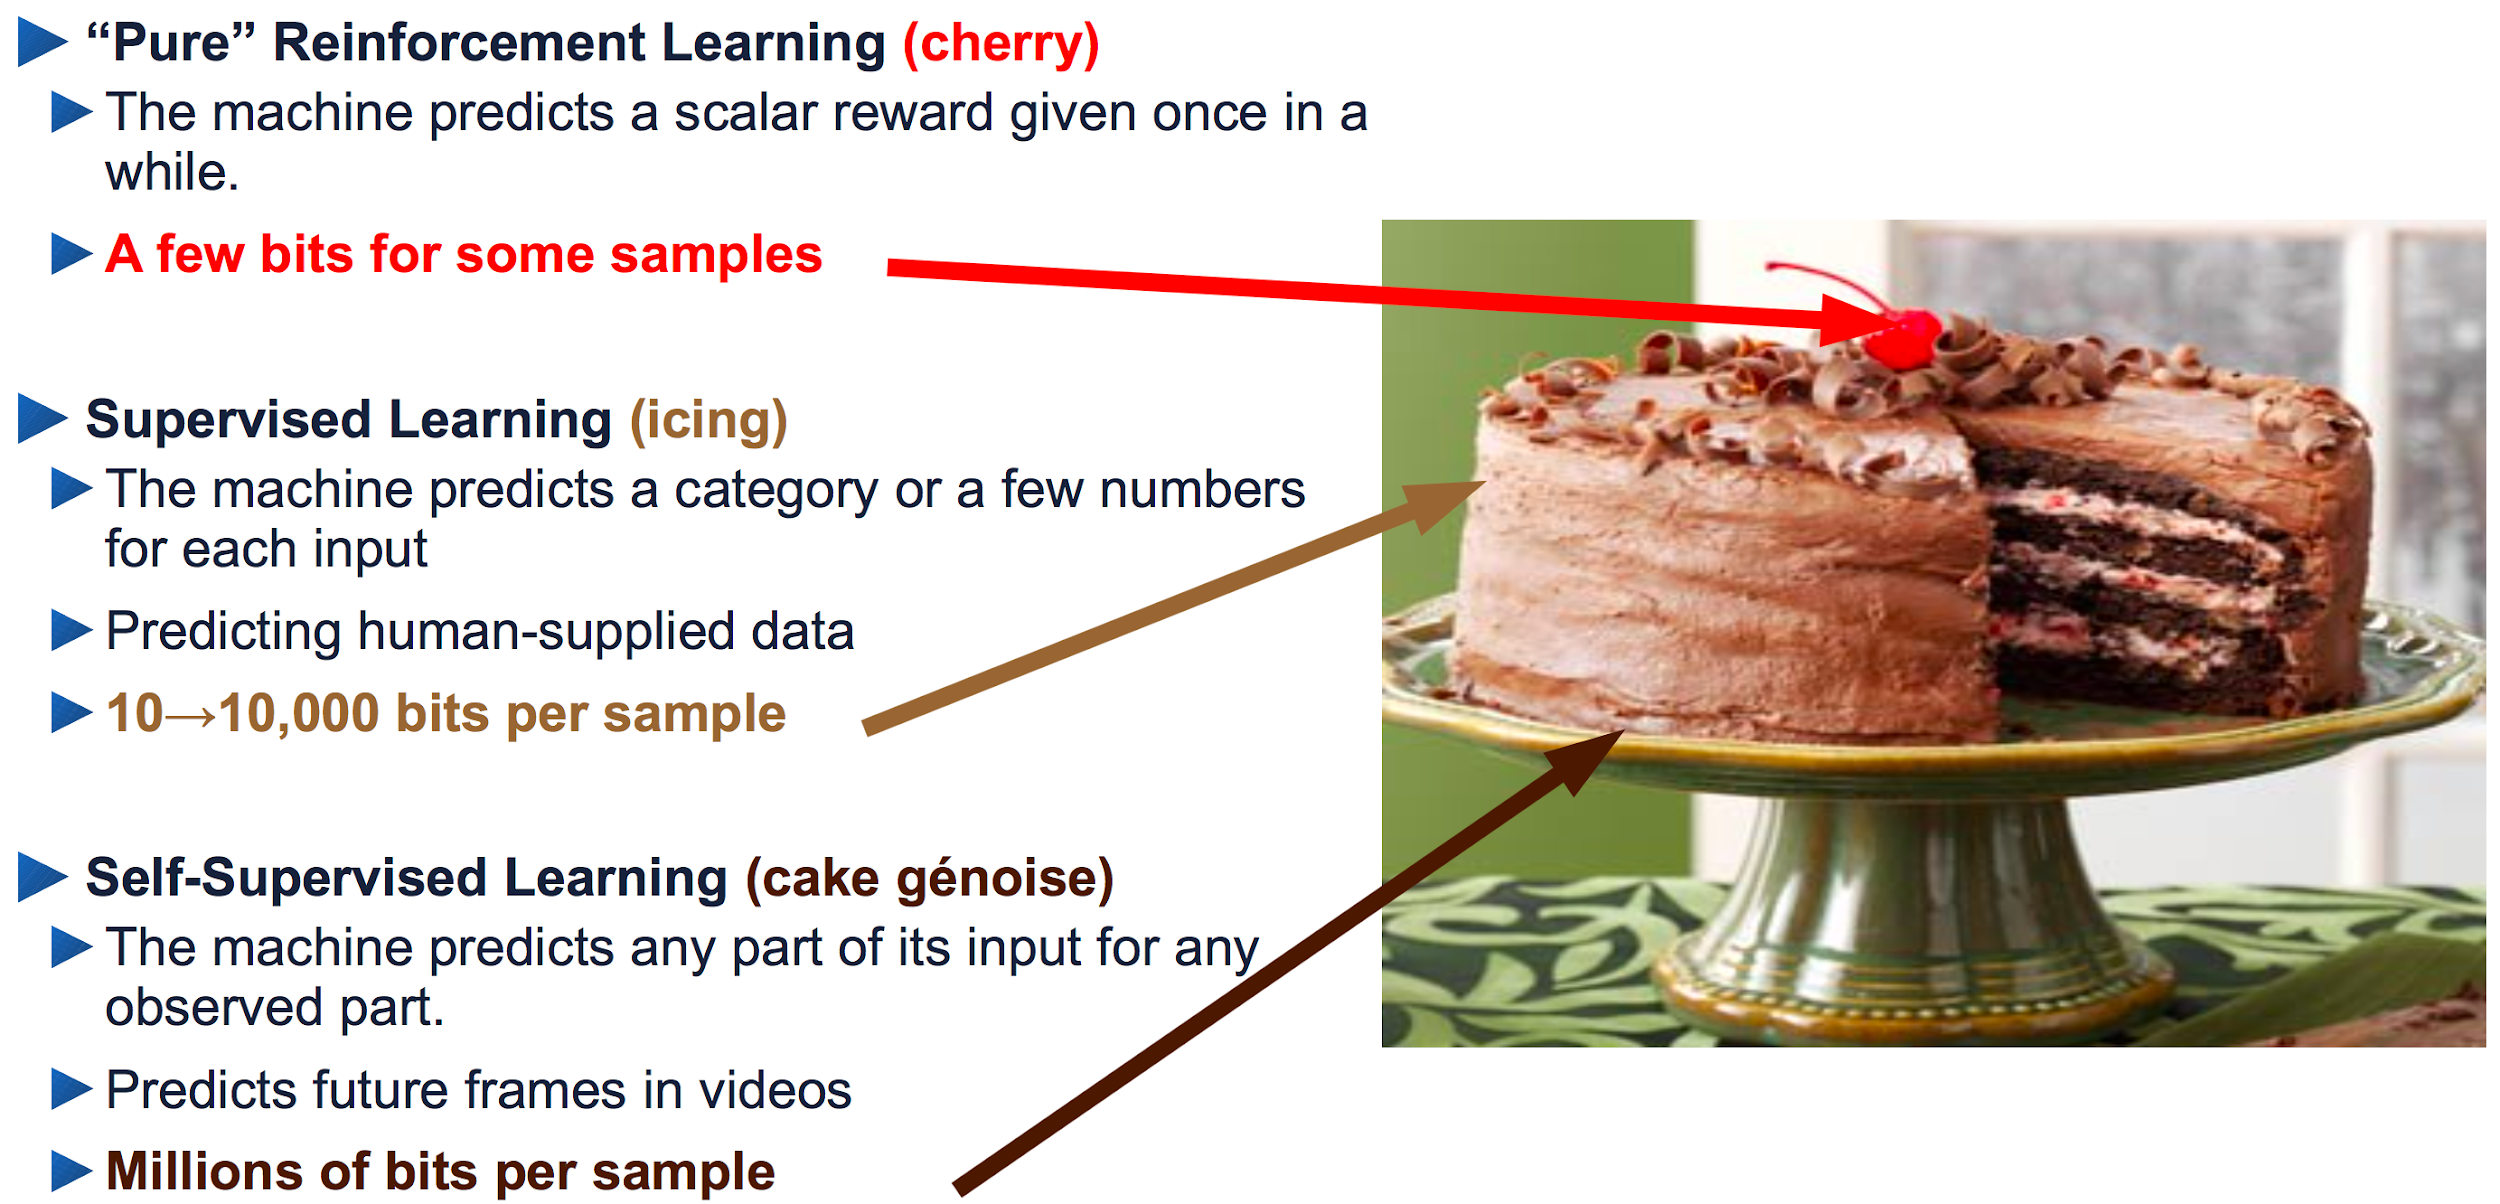
\includegraphics[width=\linewidth,height=\textheight,keepaspectratio]{images/ssl/slide_10_1_img.png}
    \end{figure}

\end{frame}